
\section{Introdução} 

 
 




\section{O Conversor VR-BESS}

O Sistema Regulador de Tensão com Armazenamento de Energia em Baterias (VR-BESS - \textit{Voltage Regulator Battery Energy Storage System}) tem como objetivo fornecer segurança e confiabilidade a sistemas de geração de energia \citep{pacheco2002dc}. Ele é composto por um conversor CC-CC de três portas, uma fonte de energia renovável ou não e uma unidade de armazenamento em baterias.

O conjunto, apresentado na Figura \ref{fig:VR-BESS}, é capaz de regular a tensão de saída, compensar oscilações de potência e de tensão de entrada. O banco de baterias permite controlar o fluxo de energia entre ele e o barramento CC, ou seja, a energia excedente produzida pela central geradora é armazenada no banco de baterias. Posteriormente, se necessário, essa energia armazenada é utilizada para suprir as necessidades da carga quando a fonte de entrada não é capaz de supri-las.




\begin{figure}[h]
\begin{center}
 
	\begin{circuitikz}[scale=0.6, font=\normalsize] [american] 
    \ctikzset{bipoles/length=6mm}
      \draw
	(0,6) to[battery1, l=$V_{in}$] (0,0)
	%(0,6) to[american inductor,l=$L_s$,f_=$i_{L_s}$] (3,6) 
    (0,6) to[american inductor,l=$L_s$] (3,6) 
	to[cute open switch, l_=$S_1$] (3,3) 
	(3,3) to[cute open switch, l_=$S_2$] (3,0) -- (0,0)
	(3,6) to [empty diode, l_=$D_3$] (5.5,6) -- (14,6);
	\draw
	(3,3) -- (5.5,3)
	(5.5,0) to[empty diode, l=$D_2$] (5.5,3)
	(5.5,3) to[empty diode, l_=$D_1$] (5.5,6)
	%(5.5,3) to[american inductor, l=$L_{bat}$, f_=$i_{L_{bat}}$]
    (5.5,3) to[american inductor, l=$L_{bat}$]
    (8.5,3) -- (10,3)
	(8.5,3) to[C, l_=$C_{bat}$] (8.5,0)
	(10,3) to[battery, l=$V_{bat}$] (10,0);
	\draw
	(12,6) to[C, l_=$C_o$](12,0)
	(14,6) to[american resistor, l_=$R_0$] (14,0) -- (0,0);
	%\draw [arrows = {-Stealth[inset=0pt, angle=50:5pt]}] (7.9,2.72) -- (7.6,2.72);
	
\end{circuitikz}  
\caption{Topologia do conversor VR-BESS} 
\label{fig:VR-BESS}
\end{center}
\end{figure}



\subsection{Principio de Funcionamento do VR-BESS}

Este conversor possui 2 modos de operação, que variam de acordo com a disponibilidade de potência nas duas fontes de alimentação presentes em seu circuito. Ele é composto de uma fonte principal ($V_{in}$) e um sistema de armazenamento de energia ($V_{bat}$). Essas duas fontes de alimentação trabalham em conjunto para realizar o balanço de potências entregue a carga, de forma que: 

\begin{itemize}
    \item \textbf{Modo 1}: a potência da fonte de entrada ($V_{in}$) é maior ou igual àquela requerida pela carga, e a bateria armazena o excedente quando este existir. O conversor VR-BESS opera como um \textit{Boost} ao elevar a tensão $V_{in}$ e regulá-la para a carga; e como um \textit{Buck} ao abaixar a tensão $V_{in}$ para carregar as baterias com $V_{bat}$;
    % \item \textbf{Modo 2}: a fonte de entrada ($V_{in}$) disponibiliza exatamente a potência requerida pela carga, não havendo necessidade do uso do sistema de armazenamento e o valor médio da corrente na bateria é zero. Neste caso, o conversor opera apenas como um \textit{Boost} ao regular a tensão para a carga;  
    \item \textbf{Modo 2}: a potência da fonte de entrada ($V_{in}$) é insuficiente ou nula e a bateria fornece o complemento da demanda da carga; Neste modo, $V_{in}$ e $V_{bat}$ atuam como dois conversores \textit{Boost} em paralelo;
    %\item \textbf{Modo 4}: nenhuma potência é fornecida pela fonte $V_{in}$ cabendo a bateria fornecer toda a potência da carga. De forma similar ao Modo 2, o conversor opera como um \textit{Boost} ao regular a tensão $V_{bat}$ para a carga.  
\end{itemize}


\subsection{Circuitos Equivalentes}

Entre os modos de operação é possível identificar cinco circuitos equivalentes diferentes. Estes circuitos estão relacionadas com os estados das chaves $S_1$ e $S_2$, com a polarização dos diodos e o sentido da corrente $I_{Lbat}$, como apresentado na Tabela \ref{tab:01}. 

\begin{table}[h]
\caption{Descrição das Etapas de Operação}
\label{tab:01}
\begin{tabular}{lllllll}
\hline
        & $S_1$ & $S_2$ & $D_1$       & $D_2$       & $D_3$       & $i_{Lbat}$ \\ \hline
Etapa 1 & 1  & 1  & Bloq. & Bloq. & Bloq. & Qualquer   \\
Etapa 2 & 1  & 0  & Bloq. & Bloq. & Conduz   & Positiva   \\
Etapa 3 & 0  & 0  & Bloq. & Conduz   & Conduz   & Positiva   \\
Etapa 4 & 0  & 0  & Conduz   & Bloq. & Conduz   & Negativa    \\
Etapa 5 & 0  & 1  & Bloq. & Bloq. & Conduz   & Negativa   \\ \hline
\end{tabular}
\end{table}

%Cabe destaque para a Etapa 3 e Etapa 4, que possuem o mesmo estado das chaves $S_1$ e $S_2$, porém o sentido da corrente $I_{Lbat}$ muda. Neste caso, a polarização de $D_1$ e $D_2$ é invertida devido ao nível de tensão da bateria em relação a fonte de alimentação e as equações são diferentes.

A dedução das equações para cada uma destas etapas é apresentada a seguir, onde é importante ressaltar que o sentido da corrente $i_{Lbat}$ que é considerado positivo é aquele que carrega a bateria. E embora o sentido da corrente mude nos circuito equivalentes ele é considerado o mesmo no momento do equacionamento, para que o modelo possa ser unificado. 

%

O circuito equivalente da Etapa 1 é apresentado na Figura \ref{fig:Modo 2 - circuito equivalente da primeira etapa}. As chaves $S_1$ e $S_2$ estão em condução e todos os diodos estão bloqueados. A partir dela pode-se definir, $L_s$ como indutor de filtro de entrada, $L_{bat}$ e $C_{bat}$ como o indutor e o capacitor de filtro da bateria e $C_0$ como capacitor de saída. Em relação às correntes e tensões, pode-se definir, $i_{Ls}$ como a corrente do indutor $L_s$, $i_{Lbat}$ a corrente do indutor $L_{bat}$, $i_{Cbat}$ e $V_{Cbat}$ como a corrente e a tensão do capacitor $C_{bat}$, $i_{C0}$ e $V_{C0}$  como a corrente e a tensão do capacitor $C_0$ e $i_{R0}$ como a corrente do resistor $R_0$.


    
    \begin{figure}[h]
    \centering
    \begin{circuitikz}[scale=0.5, font=\small] [american] 
    \ctikzset{bipoles/length=7mm}

    \draw[color=black]
    (0,6)--(0,3.1) (0,2.9)--(0,0)
    (0,6) to[american inductor, l_=$L_s$] (3,6) 
    to[cute closed switch, l_=$S_1$] (3,3) 
    (3,3) to[cute closed switch, l_=$S_2$] (3,0);
    \draw[color=gray!50]
    (3,6) to [empty diode, l_=$D_3$] (5.5,6) -- (14,6)
    (5.5,0) to[empty diode, l=$D_2$] (5.5,3)
    (5.5,3) to[empty diode, l_=$D_1$] (5.5,6);
    \draw[color=black]
    (3,3) -- (5.5,3)
    %(12,6) -- (14,6)
    (3,3) to[short] (6.5,3)
    (6.5,3) to[american inductor, l=$L_{bat}$](8.5,3) -- (11.5,3)
    (8.5,3) to[C,l_=$C_{bat}$, v^<=$V_{C{bat}}$, voltage shift=2pt] (8.5,0)
    (11.5,3)--(11.5,1.75) (11.5,1.25)--(11.5,0)
    (13.5,6) to[C, l_=$C_o$, v^<=$V_{C0}$, voltage shift=2pt] (13.5,0)
    (13.5,6) to[short] (16.5,6)
    (16.5,6) to[american resistor, l_=$R_0$] (16.5,1)-- (16.5,0)-- (0,0);
    \draw[color=black] 
    (11.5,3) to[battery, l=$V_{bat}$] (11.5,0)
    (0,6) to[battery1, l=$V_{in}$] (0,0);

   
    
     % Setas personalizadas para as correntes e tensões
    \draw[->,color=black] (2,6.3) -- (3,6.3) node[midway, above] {$i_{L_s}$};
    \draw[->,color=black] (3.5,3.2) -- (4.5,3.2) node[midway, above] {$i_{L{bat}}$};
    %\draw[->,color=black] (8,1.2) -- (8,0.2) node[midway, left] {$i_{C{bat}}$};
    \draw[->,color=black] (14,6.3) -- (15,6.3) node[midway, above] {$i_{R0}$};
    \draw[->,color=black] (13.8,5.8) -- (13.8,4.8) node[midway, right] {$i_{C0}$};



    \end{circuitikz}
    \caption{ Circuito equivalente da Etapa 1 ($S_1$=1 e $S_2$=1)} 
    \label{fig:Modo 2 - circuito equivalente da primeira etapa}
    \end{figure}

Considerando todos os elementos ideais, para simplificar a análise, e aplicando as Leis de Kirchoff das tensões e correntes, as equações diferenciais que descrevem o comportamento dinâmico podem ser obtidas como:
\begin{equation}
    \frac{d i_{Lbat}}{d t } =-\frac{v_{Cbat}}{L_{bat}} 
    \label{ModoIe1ilbat}
\end{equation}
\begin{equation}
    \frac{d i_{Ls}}{d t } =\frac{v_{in}}{L_{s}} 
    \label{ModoIe1ils}
\end{equation}
\begin{equation}
    \frac{d v_{C0}}{d t } = -\frac {v_{C0}}{C_{0}R_{0}} 
    \label{ModoIe1Vc0}
\end{equation}

A Etapa 2 é representa pela Figura \ref{fig:Modo 1 - circuito equivalente da segunda etapa}, onde a chave $S_2$ é aberta e o diodo $D_3$ passa a conduzir. As equações diferenciais que descrevem o comportamento dinâmico desta etapa são apresentadas a seguir.

  


    
%  \begin{figure}[h]
%     \centering
%     \begin{circuitikz}[scale=0.5, font=\small] [american] 
%     \ctikzset{bipoles/length=7mm}
    
%     \draw[color=black]
%     (0,6)--(0,3.1) (0,2.9)--(0,0)
%     (0,6) to[american inductor, l_=$L_s$] (3,6) 
%     to[cute closed switch, l_=$S_1$] (3,3);
%     \draw[color=gray!50]
%     (3,3) to[cute open switch, l_=$S_2$] (3,0);
%     \draw[color=black]
%     (3,6) to [empty diode, l_=$D_3$] (5.5,6) -- (14,6)
%     (3,3) -- (5.5,3);
%     \draw[color=gray!50]
%     (5.5,0) to[empty diode, l=$D_2$] (5.5,3)
%     (5.5,3) to[empty diode, l_=$D_1$] (5.5,6);
%     \draw[color=black]
%     (3,3) to[short] (6.5,3)
%     (6.5,3) to[american inductor, l=$L_{bat}$](8.5,3) -- (11.5,3)
%     (8.5,3) to[C,l_=$C_{bat}$, v^<=$V_{C{bat}}$, voltage shift=2pt] (8.5,0)
%     (11.5,3)--(11.5,1.75) (11.5,1.25)--(11.5,0)
%     (13.5,6) to[C, l_=$C_o$, v^<=$V_{C0}$, voltage shift=2pt] (13.5,0)
%     (13.5,6) to[short] (16.5,6)
%     (16.5,6) to[american resistor, l_=$R_0$] (16.5,1)-- (16.5,0)-- (0,0);
%     \draw[color=black] 
%     (11.5,3) to[battery, l=$V_{bat}$] (11.5,0)
%     (0,6) to[battery1, l=$V_{in}$] (0,0);


%      % Setas personalizadas para as correntes e tensões
%     \draw[->,color=black] (2,6.3) -- (3,6.3) node[midway, above] {$i_{L_s}$};
%     \draw[->,color=black] (3.5,3.2) -- (4.5,3.2) node[midway, above] {$i_{L{bat}}$};
%     %\draw[->,color=black] (8,1.2) -- (8,0.2) node[midway, left] {$i_{C{bat}}$};
%     \draw[->,color=black] (14,6.3) -- (15,6.3) node[midway, above] {$i_{R0}$};
%     \draw[->,color=black] (13.8,5.8) -- (13.8,4.8) node[midway, right] {$i_{C0}$};
    
% \end{circuitikz}
%  \caption{Circuito equivalente Etapa 2 ($S_1$=1 e $S_2$=0)} 
%     \label{fig:Modo 1 - circuito equivalente da segunda etapa}
%     \end{figure}

\begin{equation}
    \frac{d i_{Lbat}}{d t } =-\frac{v_{Cbat}}{L_{bat}} + \frac{v_{C0}}{L_{bat}}
    \label{ModoIe2ilbat}
\end{equation}
% \begin{equation}
%     \frac{d V_{Cbat}}{d t } = \frac {i_{Lbat}}{C_{bat}} - \frac {V_{Cbat}}{C_{bat}R_{bat}} 
%     \label{ModoIe2Vcbat}
% \end{equation}
\begin{equation}
    \frac{d i_{Ls}}{d t } = \frac{v_{in}}{L_s} -\frac{v_{C0}}{L_{s}}  
    \label{ModoIe2ils}
\end{equation}
\begin{equation}
    \frac{d v_{C0}}{d t } = -\frac{i_{Lbat}}{C_0} + \frac{i_{Ls}}{C_0}  -\frac {v_{C0}}{C_{0}R_{0}} 
    \label{ModoIe2Vc0}
\end{equation}


A Etapa 3, apresentada na Figura \ref{fig:Modo 2 - circuito equivalente da terceira etapa}, ocorre quando a chave $S_1$ e $S_2$ são aberta e a corrente $I_{Lbat}>0$. As equações diferenciais que descrevem o comportamento dinâmico desta etapa são apresentadas a seguir.

% \begin{figure} [h]
 %   \begin{center}
  %  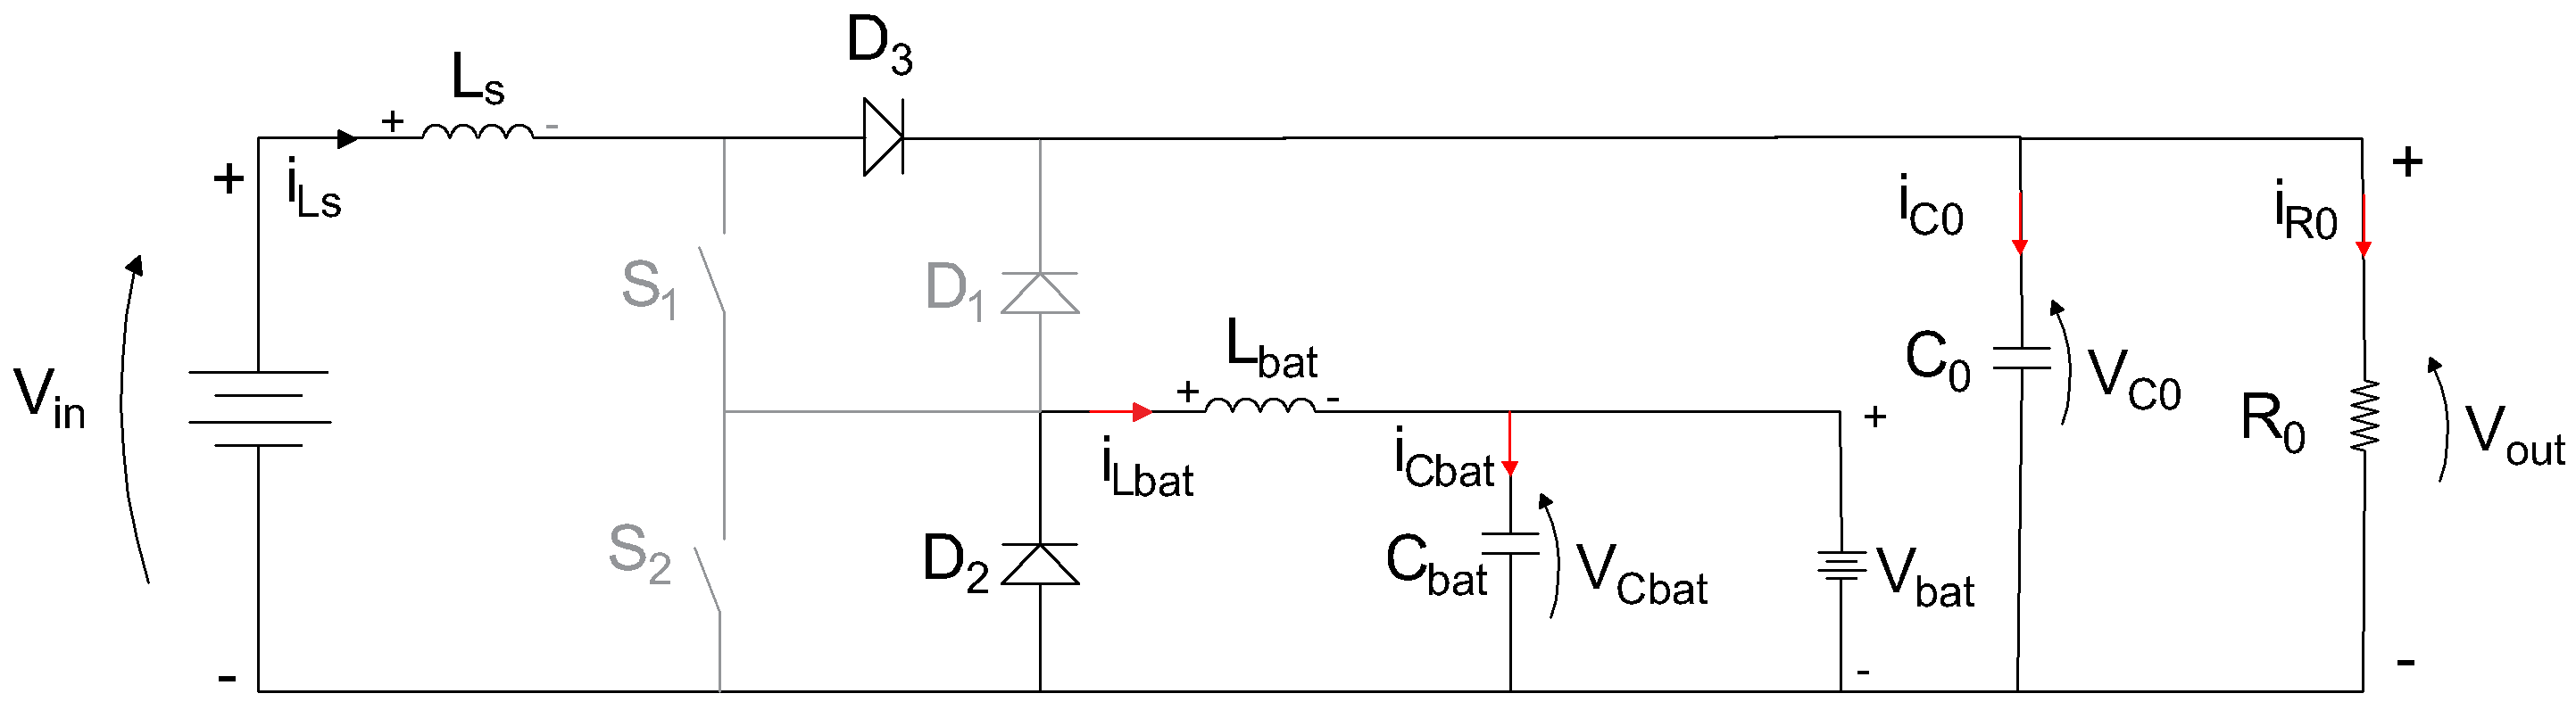
\includegraphics[width=\linewidth]{Figuras/VrbessM2e2.png}   
   % \caption{ Circuito Equivalente Etapa 3 ($S_1$=0 e $S_2$=0)} 
    %\label{fig:Modo 2 - circuito equivalente da terceira etapa}
    %\end{center}
%\end{figure}

% \begin{figure}[h]
%     \centering
%     \begin{circuitikz}[scale=0.5, font=\small] [american] 
%     \ctikzset{bipoles/length=7mm}
    
%    \draw[color=black]
%     (0,6)--(0,3.1) (0,2.9)--(0,0)
%     (0,6) to[american inductor, l_=$L_s$] (3,6);
%     \draw[color=gray!50]
%     (3,3) -- (5.5,3)
%     (3,6) to[cute open switch, l_=$S_1$] (3,3) 
%     (3,3) to[cute open switch, l_=$S_2$] (3,0);
%     \draw[color=black]
%     (3,6) to [empty diode, l_=$D_3$] (5.5,6) -- (14,6)
%     (5.5,0) to[empty diode, l=$D_2$] (5.5,3);
%     \draw[color=gray!50]
%     (5.5,3) to[empty diode, l_=$D_1$] (5.5,6);
%     \draw[color=black]
%     (5.5,3) to[short] (6.5,3)
%     (6.5,3) to[american inductor, l=$L_{bat}$](8.5,3) -- (11.5,3)
%     (8.5,3) to[C,l_=$C_{bat}$, v^<=$V_{C{bat}}$, voltage shift=2pt] (8.5,0)
%     (11.5,3)--(11.5,1.75) (11.5,1.25)--(11.5,0)
%     (13.5,6) to[C, l_=$C_o$, v^<=$V_{C0}$, voltage shift=2pt] (13.5,0)
%     (13.5,6) to[short] (16.5,6)
%     (16.5,6) to[american resistor, l_=$R_0$] (16.5,1)-- (16.5,0)-- (0,0);
%     \draw[color=black] 
%     (11.5,3) to[battery, l=$V_{bat}$] (11.5,0)
%     (0,6) to[battery1, l=$V_{in}$] (0,0);

%       % Setas personalizadas para as correntes e tensões
%     \draw[->,color=black] (2,6.3) -- (3,6.3) node[midway, above] {$i_{L_s}$};
%     \draw[->,color=black] (5.8,2.7) -- (6.8,2.7) node[midway, below] {$i_{L{bat}}$};
%     %\draw[->,color=black] (8,1.2) -- (8,0.2) node[midway, left] {$i_{C{bat}}$};
%     \draw[->,color=black] (14,6.3) -- (15,6.3) node[midway, above] {$i_{R0}$};
%     \draw[->,color=black] (13.8,5.8) -- (13.8,4.8) node[midway, right] {$i_{C0}$};

    
% \end{circuitikz}
%  \caption{ Circuito Equivalente Etapa 3 ($S_1$=0 e $S_2$=0)} 
%     \label{fig:Modo 2 - circuito equivalente da terceira etapa}
% \end{figure}

% \begin{equation}
%     \frac{d i_{Lbat}}{d t } =-\frac{v_{Cbat}}{L_{bat}} 
%     \label{ModoIe2ilbat}
% \end{equation}
% \begin{equation}
%     \frac{d i_{Ls}}{d t } = \frac{v_{in}}{L_s} -\frac{v_{C0}}{L_{s}}  
%     \label{ModoIe2ils}
% \end{equation}
% \begin{equation}
%     \frac{d v_{C0}}{d t } = \frac{i_{Ls}}{C_0} -\frac {v_{C0}}{C_{0}R_{0}} 
%     \label{ModoIe2Vc0}
% \end{equation}




A Etapa 4 está representada na Figura \ref{fig:Modo 3 - circuito equivalente da terceira etapa}, e ocorre também quando a chave $S_1$ e $S_2$ são abertas, porém a corrente $I_{Lbat}<0$. O comportamento dinâmico da Etapa 4 pode ser descrito pelas equações diferenciais seguintes.


%\begin{figure}[h]
 %   \begin{center}
  %  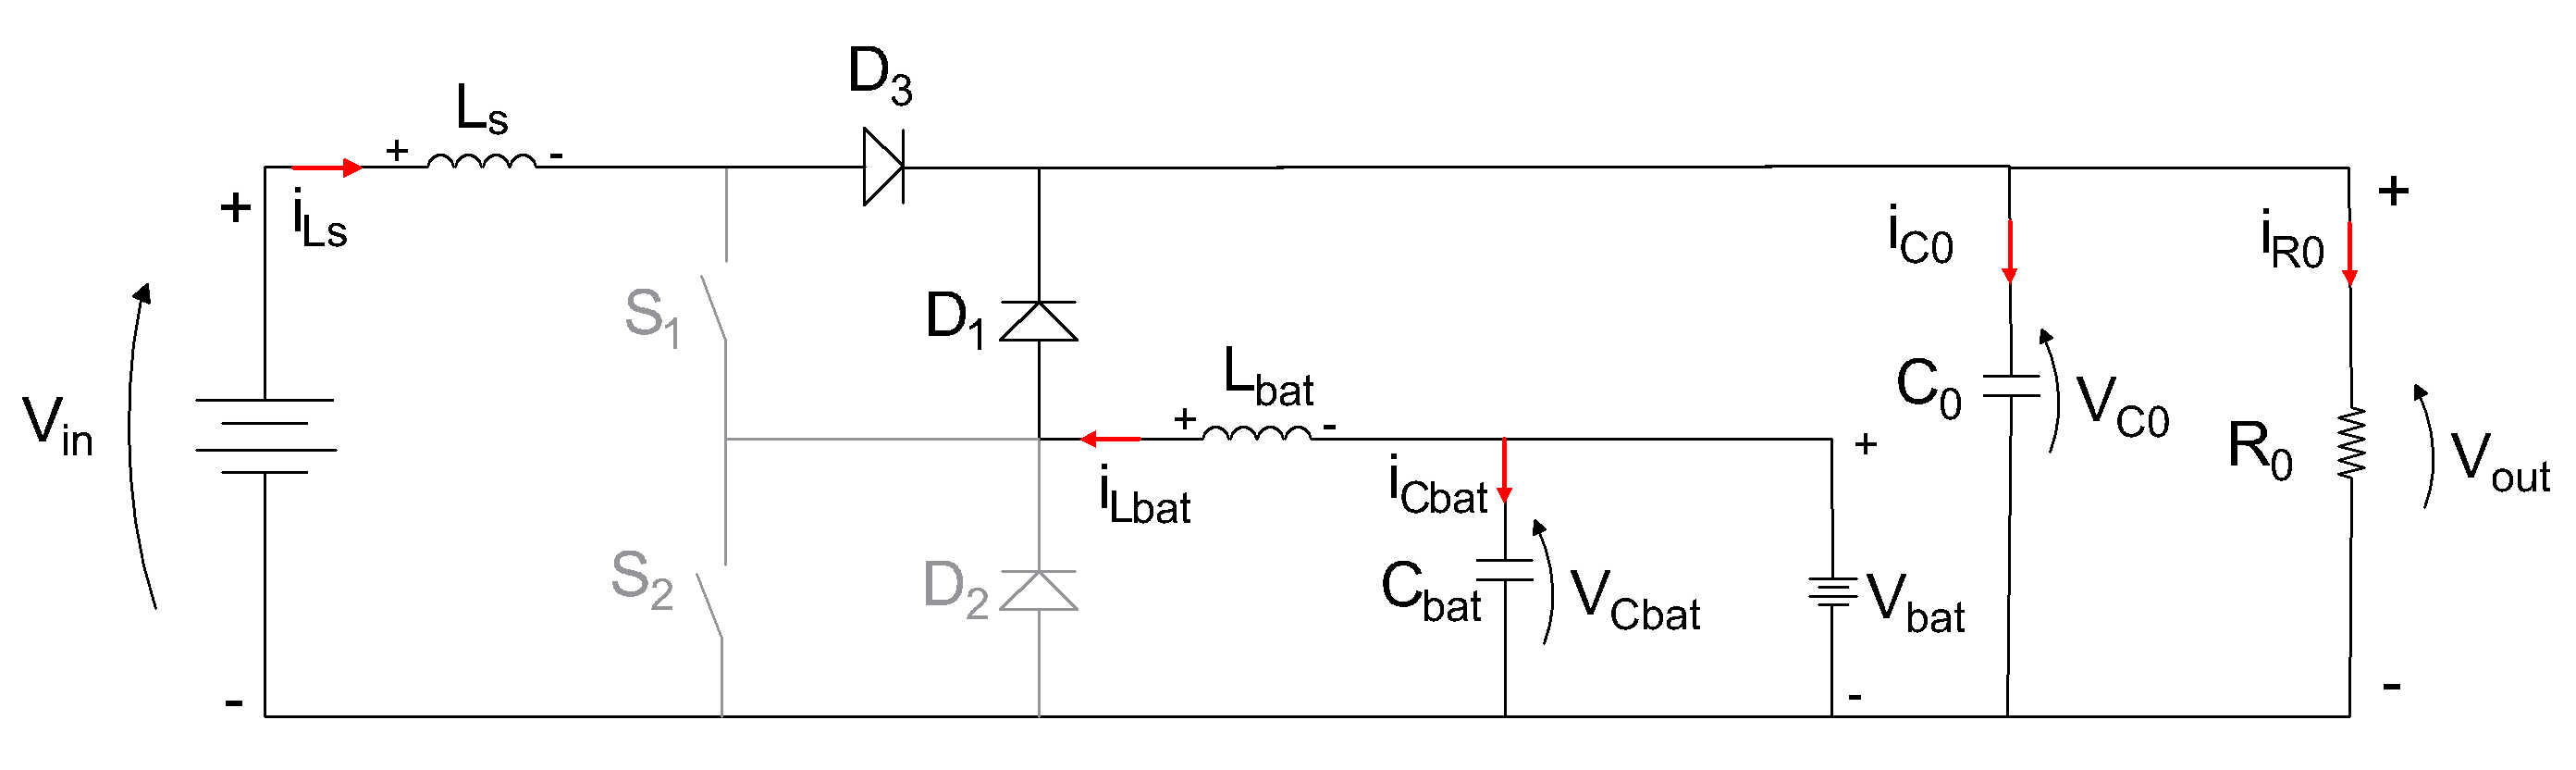
\includegraphics[width=\linewidth]{Figuras/ETAPA 3.png}
   % \caption{Circuito equivalente da Etapa 4 ($S_1$=0 e $S_2$=0)} 
    %\label{fig:Modo 3 - circuito equivalente da terceira etapa}
    %\end{center}
%\end{figure}

% \begin{figure}[h]
% \centering
%     \begin{circuitikz}[scale=0.5, font=\small] [american] 
%     \ctikzset{bipoles/length=7mm}
    
%    \draw[color=black]
%     (0,6)--(0,3.1) (0,2.9)--(0,0)
%     (0,6) to[american inductor, l_=$L_s$] (3,6);
%     \draw[color=gray!50]
%     (3,3) -- (5.5,3)
%     (3,6) to[cute open switch, l_=$S_1$] (3,3) 
%     (3,3) to[cute open switch, l_=$S_2$] (3,0);
%     \draw[color=black]
%     (3,6) to [empty diode, l_=$D_3$] (5.5,6) -- (14,6);
%     \draw[color=gray!50]
%     (5.5,0) to[empty diode, l=$D_2$] (5.5,3);
%     \draw[color=black]
%     (5.5,3) to[empty diode, l_=$D_1$] (5.5,6)
%     (5.5,3) to[short] (6.5,3)
%     (6.5,3) to[american inductor, l=$L_{bat}$](8.5,3) -- (11.5,3)
%     (8.5,3) to[C,l_=$C_{bat}$, v^<=$V_{C{bat}}$, voltage shift=2pt] (8.5,0)
%     (11.5,3)--(11.5,1.75) (11.5,1.25)--(11.5,0)
%     (13.5,6) to[C, l_=$C_o$, v^<=$V_{C0}$, voltage shift=2pt] (13.5,0)
%     (13.5,6) to[short] (16.5,6)
%     (16.5,6) to[american resistor, l_=$R_0$] (16.5,1)-- (16.5,0)-- (0,0);
%     \draw[color=black] 
%     (11.5,3) to[battery, l=$V_{bat}$] (11.5,0)
%     (0,6) to[battery1, l=$V_{in}$] (0,0);

%       % Setas personalizadas para as correntes e tensões
%     \draw[->,color=black] (2,6.3) -- (3,6.3) node[midway, above] {$i_{L_s}$};
%     \draw[<-,color=black] (5.8,2.7) -- (6.8,2.7) node[midway, below] {$i_{L{bat}}$};
%     \draw[->,color=black] (14,6.3) -- (15,6.3) node[midway, above] {$i_{R0}$};
%     \draw[->,color=black] (13.8,5.8) -- (13.8,4.8) node[midway, right] {$i_{C0}$};

    
% \end{circuitikz}
%     \caption{Circuito equivalente da Etapa 4 ($S_1$=0 e $S_2$=0)} 
%     \label{fig:Modo 3 - circuito equivalente da terceira etapa}
% \end{figure}

\begin{equation}
    \frac{d i_{Lbat}}{d t } =-\frac{v_{Cbat}}{L_{bat}}+\frac{v_{C0}}{L_{bat}}
    \label{ModoIIe3ilbat}
\end{equation}
\begin{equation}
    \frac{d i_{Ls}}{d t } =\frac{v_{in}}{L_{s}}-\frac{v_{C0}}{L_{s}}
    \label{ModoIIe3ils}
\end{equation}
\begin{equation}
    \frac{d v_{C0}}{d t } =-\frac{i_{Lbat}}{C_0}+ \frac{i_{Ls}}{C_0} -\frac {v_{C0}}{C_{0}R_{0}} 
    \label{ModoIIe3Vc0}
\end{equation}


Por fim, a Etapa 5 é representada pela Figura \ref{fig:Modo 3 - circuito equivalente da segunda etapa}, que apresenta o momento em que a chave $S_1$ é aberta e $S_2$ é fechada.  As equações diferenciais que descrevem o comportamento desta etapa são apresentadas a seguir.

%\begin{figure}[h]
 %   \begin{center}
  %  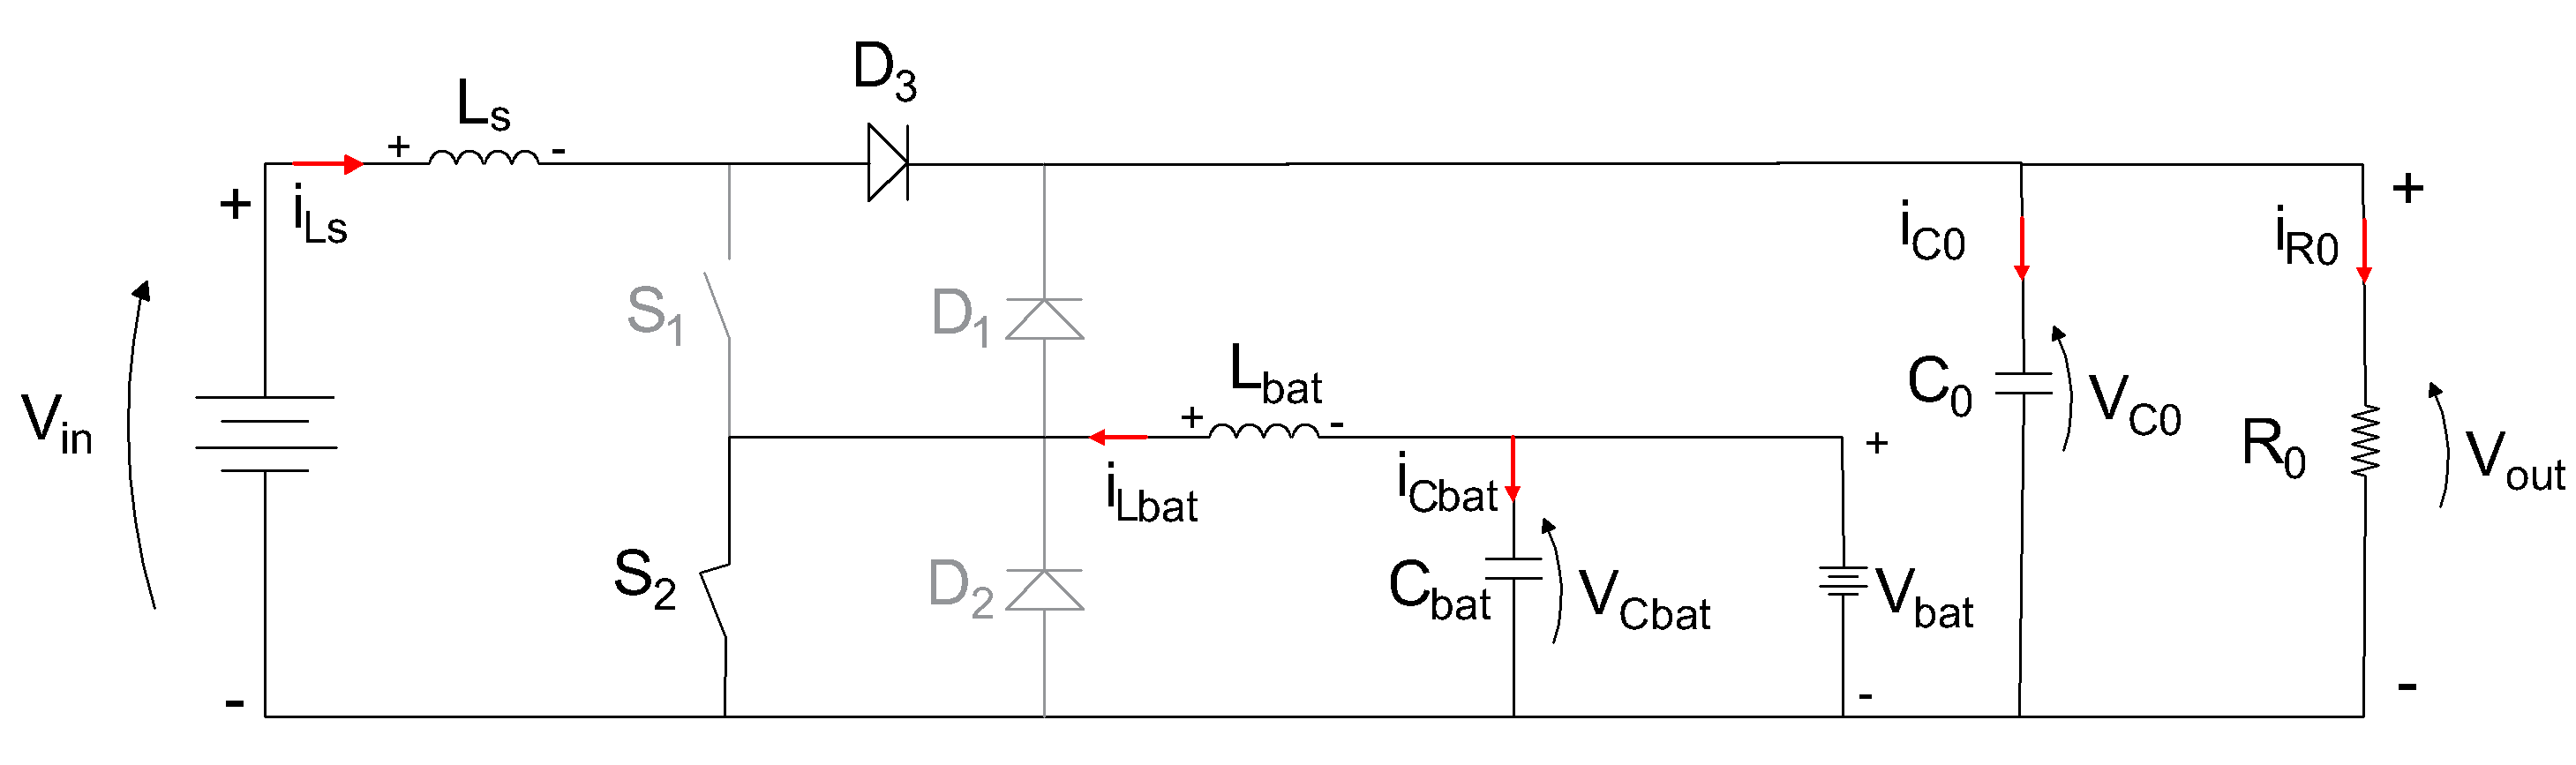
\includegraphics[width=\linewidth]{Figuras/ETAPA 2.png}
   % \caption{Circuito equivalente da Etapa 5 ($S_1$=0 e $S_2$=1)} 
    %\label{fig:Modo 3 - circuito equivalente da segunda etapa}
    %\end{center}
%\end{figure}

\begin{figure}[h]
    \centering
    \begin{circuitikz}[scale=0.5, font=\small] [american] 
    \ctikzset{bipoles/length=7mm}
    
    \draw[color=black]
    (0,6)--(0,3.1) (0,2.9)--(0,0)
    (0,6) to[american inductor, l_=$L_s$] (3,6);
    \draw[color=gray]
    (3,6) to[cute open switch, l_=$S_1$] (3,3);
    \draw[color=black]
    (3,3) to[cute closed switch, l_=$S_2$] (3,0)
    (3,6) to [empty diode, l_=$D_3$] (5.5,6) -- (14,6)
    (3,3) -- (6.5,3);
    \draw[color=gray]
    (5.5,0) to[empty diode, l=$D_2$] (5.5,3)
    (5.5,3) to[empty diode, l_=$D_1$] (5.5,6.0);
    \draw[color=black]
    (6.5,3) to[american inductor, l=$L_{bat}$](8.5,3) -- (11.5,3)
    (8.5,3) to[C,l_=$C_{bat}$, v^<=$V_{C{bat}}$, voltage shift=2pt] (8.5,0)
    (11.5,3)--(11.5,1.75) (11.5,1.25)--(11.5,0)
    (13.5,6) to[C, l_=$C_o$, v^<=$V_{C0}$, voltage shift=2pt] (13.5,0)
    (13.5,6) to[short] (16.5,6)
    (16.5,6) to[american resistor, l_=$R_0$] (16.5,1)-- (16.5,0)-- (0,0);
    \draw[color=black] 
    (11.5,3) to[battery, l=$V_{bat}$] (11.5,0)
    (0,6) to[battery1, l=$V_{in}$] (0,0);


    % Setas personalizadas para as correntes e tensões
    \draw[->,color=black] (2,6.3) -- (3,6.3) node[midway, above] {$i_{L_s}$};
    \draw[<-,color=black] (5.8,2.7) -- (6.8,2.7) node[midway, below] {$i_{L{bat}}$};
    \draw[->,color=black] (14,6.3) -- (15,6.3) node[midway, above] {$i_{R0}$};
    \draw[->,color=black] (13.8,5.8) -- (13.8,4.8) node[midway, right] {$i_{C0}$};

    
\end{circuitikz}
 \caption{Circuito equivalente da Etapa 5 ($S_1$=0 e $S_2$=1)} 
    \label{fig:Modo 3 - circuito equivalente da segunda etapa}
\end{figure}

\begin{equation}
    \frac{d i_{Lbat}}{d t } =-\frac{v_{Cbat}}{L_{bat}} 
    \label{ModoIe3ilbat}
\end{equation}
\begin{equation}
    \frac{d i_{Ls}}{d t } =\frac{v_{in}}{L_s} -\frac{v_{C_0}}{L_{s}}  
    \label{ModoIe3ils}
\end{equation}
\begin{equation}
    \frac{d v_{C_0}}{d t } = \frac{i_{Ls}}{C_0}-\frac {v_{C0}}{C_{0}R_{0}} 
    \label{ModoIe3Vc0}
\end{equation}





\subsection{Modelo Unificado do VR-BESS} 

No trabalho de \cite{marcello22019modelagem}, os autores apresentaram um modelo para cada modo de operação utilizando a técnica de modelo médio em espaço de estados. Entretanto, o FCS-MPC utiliza um modelo matemático discreto em função dos estados de chaveamento ($S_1$ e $S_2$). Dessa forma, o objetivo deste trabalho é apresentar um modelo unificado discreto para os quatro modos de operação em função destes estados de chaveamento. Para tanto, a metodologia utilizada para obtenção desse modelo toma como base as equações diferenciais apresentadas na sessão anterior. As diferenças entre cada uma delas é identificada visando encontrar uma relação lógica com os estados de chaveamento. Os seguintes critérios são propostos: 

\begin{itemize}
    \item Para as Etapas 3 e 4 uma variável binária  $\lambda$ é criada pra indicar a mudança no sentido da corrente $i_{Lbat}$ em um mesmo estado de chaveamento $S_1=0$ e $S_2=0$; 
    \item Para as equações de $i_{Lbat}$, as diferenças são mapeadas em função da existência do termo $\dfrac{v_{C0}}{L_{bat}}$; 
    \item Para as equações de $i_{Ls}$, as diferenças são avaliadas em função do termo $\dfrac{v_{C0}}{L_{s}}$;
    \item Para as equações de $v_{C0}$, as diferenças são mapeadas em função dos termos $\dfrac{i_{Ls}}{C_0}$ e $\frac{i_{Lbat}}{C_0}$.
\end{itemize}

Essas diferenças são resumidas de forma lógica, na Tabela (\ref{ConjuntoChaves}), onde 1 indica a existência do termo e 0 indica sua ausência. Na sequência, uma expressão lógica é obtida  para cada termo descrito. As expressões são obtidas por meio da análise de um Mapa de Karnaugh, onde as entradas, são os estados da chave $S_1$, $S_2$ e a variável $\lambda$ e a saída é cada termo em discussão. 



\begin{table}[h]
\caption{Mapeamento de Termos das Equações Diferenciais para Análise Lógica}
\label{ConjuntoChaves}
\begin{tabular}{cccc|cccc}
\hline
          & \multicolumn{3}{c}{Entradas}         & \multicolumn{4}{c}{Saídas}                                                                        \\ \hline
          & S1   & S2  & $\lambda$  & $\dfrac{v_{C0}}{L_{bat}}$ & $\dfrac{v_{C0}}{L_{s}}$ & $\dfrac{i_{Lbat}}{C_0}$ & $\frac{i_{Ls}}{C_0}$ \\ \hline
Etapa 1   & 1    & 1   & 0                       & 0                        & 0                      & 0                    & 0                      \\
Etapa 2   & 1    & 0   & 0                       & 1                        & 1                      & 1                    & 1                      \\
Etapa 3   & 0    & 0   & 0                       & 0                        & 1                      & 0                   & 1                      \\
Etapa 4   & 0    & 0   & 1                       & 1                        & 1                      & 1                    & 1                      \\
Etapa 5   & 0    & 1   & 0                       & 0                        & 1                      & 0                    & 1                      \\ \hline
\multicolumn{4}{c}{Expressões lógicas} & $\gamma$     & 1-$S_1$$S_2$                   & $\gamma$                 & 1-$S_1$$S_2$   \\ \hline
\end{tabular}
\end{table}


Onde $\gamma = S_1(1 - S_2)+ \lambda(1-S_1)(1-S_2)$.

A partir das expressões lógicas obtidas na Tabela \ref{ConjuntoChaves}, o modelo unificado em espaço de estados pode ser definido como:
$$
\begin{bmatrix}
\dot{i}_{Lbat} \\
\dot{i}_{Ls}\\
\dot{v}_{C0}\\

\end{bmatrix} =
\begin{bmatrix}
0 & 0 & \frac{\gamma}{L_{bat}}\\
0 & 0 & -\frac{(1-S_1S_2)}{L_s}\\
-\frac{\gamma}{C_o} & \frac{(1-S_1S_2)}{C_o} & -\frac{1}{R_oC_o}\\
\end{bmatrix} 
\begin{bmatrix}
i_{Lbat} \\
i_{Ls}\\
v_{C0}
\end{bmatrix} 
$$
$$
+ 
\begin{bmatrix}
0 & -\frac{1}{L_{bat}}\\
\frac{1}{L_s} & 0\\
0 & 0
\end{bmatrix} 
\begin{bmatrix}
v_{in}\\
v_{Cbat}\\
\end{bmatrix} 
$$
Por fim, o modelo contínuo pode ser pode ser discretizado por meio das aproximações:

\begin{equation}
    \centering
    x(k+1) = A_d x(k) + B_d u(k)
\label{discretizando}
\end{equation}
\begin{equation}
    \centering
    A_d = e^{AT_s} \approx I+\frac{AT_s}{1!}
\label{Ad}
\end{equation}
\begin{equation}
    \centering
    B_d\approx BT_s
\label{Bd}
\end{equation}


\noindent onde, $x$ é a variável de estado do sistema, $u$ é a entrada do sistema, $k$ é um múltiplo inteiro do período de amostragem ($t=kT_s$), $A$ é a matriz de estados do sistema contínuo, $B$ é a matriz de entradas e $I$ é uma matriz identidade. A matriz de estados discreta $A_d$ e a matriz de entrada $B_d$ são resultantes da aproximação definida em (\ref{Ad}) e (\ref{Bd}).


 




\section{Aplicação do FCS-MPC no VR-BESS} 




As etapas do algoritmo implementado para execução do FCS-MPC são apresentadas a seguir. 

\begin{itemize}
    \item Medição das variáveis, que incluem as tensões $v_{in}$, $v_{Cbat}$ e $v_{C0}$ e as correntes $i_{Ls}$ e $i_{Lbat}$;
    \item Obtenção do modelo discreto em função dos estados de chaveamento; 
    \item Predição das variáveis de estado utilizando o modelo discreto proposto; 
    \item Definição do modo de operação e consequentemente do valor da variável $\lambda$;
    \item Cálculo das referências $i_{Ls}^*$ e $i_{Lbat}^*$, em função do modo de operação;
    \item Definição dos estados ótimos $S_{1_{opt}}$ e $S_{2_{opt}}$ ao conversor VR-BESS, por meio da avaliação da Função Custo. 
\end{itemize}



De acordo com o princípio básico de operação do FCS-MPC, as três etapas principais para seu funcionamento são: definição de um modelo discreto, definição das referências e definição da função custo. As duas últimas etapas serão descritas em detalhes na sessão seguinte.

\subsection{Definição da Função Custo}

O conversor VR-BESS pode operar aliando o modo de funcionamento dos conversores \textit{Buck} e \textit{Boost}, apenas do conversor \textit{Boost}, e também como dois conversores \textit{Boost}. Sendo assim, no geral os objetivos de controle deste sistema podem ser: 

\begin{itemize}
    \item Controle das tensões $V_{Cbat}$ e $V_{C0}$ de forma indireta por meio das correntes $i_{Ls}$ e $i_{Lbat}$;
    \item Controle direto das tensões $V_{Cbat}$ e $V_{C0}$.
%    \item Controle multivariável das tensões $V_{Cbat}$ e $V_{C0}$ e das correntes $i_{Ls}$ e $i_{Lbat}$.
\end{itemize}

Essas possibilidades foram avaliadas para o conversor \textit{Boost} e os resultados discutidos em \cite{braga2022controle}. O conversor VR-BESS, por sua vez, tem seu princípio de operação derivado do conversor \textit{Boost} e para o controle direto de tensões este é um conversor que possui características de Fase não Mínima (FNM). 

Como discutido em \cite{braga2022controle}, o controle direto da tensão necessita de adequações na função custo para obter resultados satisfatórios. Por outro lado, o controle indireto da tensão, utilizando funções custo de corrente, apresentou bons resultados com pequenos desvios em regime permanente. Dessa forma, para evitar a necessidade de correções na função custo devido a FNM, optou-se por realizar o controle indireto de tensão, por meio da função custo com as correntes $i_{Ls}$ e $i_{Lbat}$. 

A função custo quadrática para o controle indireto das tensões ($g_i$) pode ser definida de forma geral como : 
\begin{equation}
    g_i = [i^*_{Ls}-i_{Ls}(k+2)]^2 + [i^*_{Lbat}-i_{Lbat}(k+2)]^2
\end{equation}


\noindent onde $i^*_1$ e $i^*_2$ são os valores de referência para as correntes, e $i_1(k+2)$ e $i_2(k+2)$ são os valores das correntes preditos pelo FCS-MPC por meio do modelo discreto. De acordo com \cite{delay}, o horizonte de predição de duas amostras é utilizado visando compensar o atraso causado entre o cálculo do algoritmo e a aplicação dos estados na chave. Dessa forma, no primeiro instante de predição é compensado o tempo de processamento do algoritmo e no segundo são previstas as variáveis de estado. 

\subsection{\textcolor{red}{Definição das Referências de Controle} }


% O objetivo de controle em cada modo de operação é garantir uma tensão regulada na saída  de forma que $V^*_{C0} =400V$, $i^*_{Lbat} = 1,08A$ para carga e $i^*_{Lbat}=-1,08A$ para descarga da bateria, valores predefinidos como características do projeto. 

% Desta forma, para garantir o controle indireto destas tensões, ao acrescentar as correntes $i_{Ls}$ e $i_{Lbat}$ nas funções custo é preciso calcular os valores de referência a serem utilizados para estas variáveis, sendo estes $i^*_{Ls}$ e $i^*_{Lbat}$, respectivamente.  Os cálculos são feitos por meio do balanço de potência de entrada e saída (desprezando as perdas), de forma que para o Modo 1 as referências são dadas por:

As referências de controle serão obtidas por meio do balanço de potências, de forma que: 

\begin{equation}
    P_{carga} = P_{bat} + P_{PV}    
\end{equation}

onde, 

\begin{equation}
    P_{carga} =  \frac{(V^*_{C0})^2}{R_o}  
\end{equation}

e 

\begin{equation}
    P_{PV} =  P_{Max}  
\end{equation}

A $P_{Max}$ é a máxima potência fornecida pelo painel fotovoltaico para uma dada irradiância. Ela pode ser obtida por meio de um algoritmo de rastreamento de máxima potência ou a partir da folha de dados do painel. Para cada valor de $P_{Max}$, estão associadas uma corrente $I_{MP}$ e uma tensão $V_{MP}$. Em um primeiro momento, não será utilizado o algoritmo de rastreamento. A referência de corrente do painel ($i_{Ls}^*$) será obtida diretamente da folha de dados, e será dada por:

\begin{equation}
    i_{Ls}^* = I_{MP}
\end{equation}

Já a referência de corrente da bateria é obtida isolando a potência da bateria

\begin{equation}
i_{Lbat}^* = \bigg(\frac{P_{carga} - P_{PV}}{V_{Cbat}} \bigg)
\end{equation}




\subsection{Restrições em Cada Modo de Operação}

\textcolor{red}{Manter as restrições apenas do modo 1 (que agora junta modo 1 e 2), e modo 3 (que agora junta modo 3 e modo 4) e é chamado de modo 2}

Para que o controlador encontre o estado ótimo de chaveamento em cada passo é necessário que algumas restrições sejam seguidas. Restringir cada modo à suas respectivas etapas, portanto o \textbf{Modo 1} opera as Etapas 1, 2 e 3, o \textbf{Modo 2} opera as Etapas 1 e 3, o \textbf{Modo 3} opera as Etapas 1, 4 e 5, e o \textbf{Modo 4} as Etapas 4 e 5. A variável $\lambda$ deve ser 1 para os \textbf{Modos 3 e 4}.

\section{Resultados}

Nesta seção, os resultados da simulação realizada no software \textit{Matlab/Simulink} são apresentados para demonstrar o desempenho do controle FCS-MPC em cada modo de operação. Utiliza-se o bloco do Simulink chamado \textit{S-Function} para a implementação em linguagem C do algoritmo de controle, onde o modelo unificado proposto é utilizado juntamente com os parâmetros apresentados na Tabela~\ref{tab:parâmetrosVRBESS}.


\begin{table}[htb]
\begin{center}
\caption{Parâmetros de Simulação.}
\begin{tabular}{ccc} \hline
\textbf{Símbolo} & \textbf{Descrição} & \textbf{Valor} \\\hline
$L_s$ & Indutor do filtro de entrada & $3,5mH$ \\
$C_0$ & Capacitor do filtro de saída  & $400\mu F$  \\ 
$R_0$ & Resistência (carga) & $160\Omega$ \\
$L_{bat}$ & Indutor do filtro da bateria & $3mH$ \\
$C_{bat}$ & Capacitor do filtro da bateria  & $500\mu F$  \\
$f_s$ & Frequência de amostragem & $100kHz$ \\
$V_{in}$ & Tensão de entrada & $300V$ \\
\hline
\end{tabular}
 \vspace{10pt}
 \label{tab:parâmetrosVRBESS}
\end{center}
\end{table} 


\begin{figure*}[t]
    \centering
    \begin{subfigure}[b]{0.45\linewidth}
        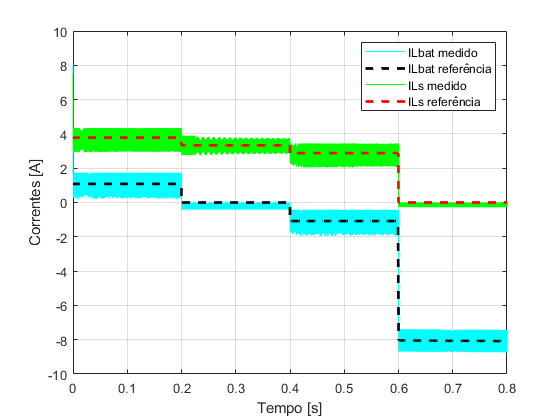
\includegraphics[width=\linewidth]{Figuras/Correntes_resultados_grid.png}
        %\caption{$I_{Ls}$ e $I_{Lbat}$}
    \end{subfigure}
    \hfill % Espaço entre as subfiguras
    \begin{subfigure}[b]{0.45\linewidth}
        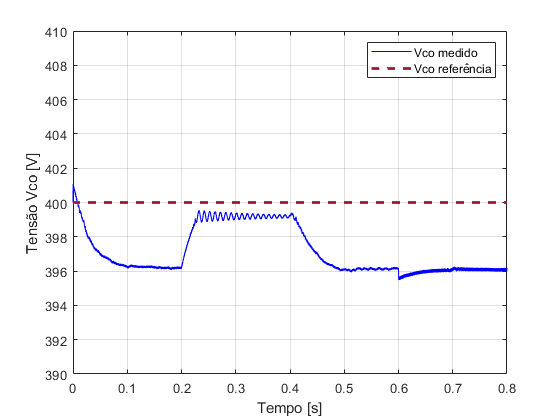
\includegraphics[width=\linewidth]{Figuras/Vco_resultados_grid.png}
        %\caption{$V_{co}$} 
    \end{subfigure}
    \caption{Resultados das medições nos quatro modos de operação de (a) correntes $i_{Ls}$ e $i_{Lbat}$ e (b) tensão $v_{co}$}
    \label{fig:resultadosVco}
\end{figure*}


\begin{table*}[h]
\begin{center}
\caption{Valores médios, erro médio em regime permanente e oscilação de $i_{Ls}$, $i_{Lbat}$ e $v_{co}$.}
\begin{tabular}{ c *{4}{c} *{4}{c} *{4}{c} }
\hline
\multicolumn{1}{c|}{} & \multicolumn{4}{c|}{$i_{Ls}$} & \multicolumn{4}{c|}{$i_{Lbat}$} & \multicolumn{4}{c}{$v_{co}$} \\ 
\hline 
 Modo &  Ref.[A] & $\Bar{i_{Ls}}$ [A] & EMRP & $\Delta i_{Ls}$[A] & Ref.[A] & $\Bar{i_{Lbat}}$ [A] & EMRP & $\Delta i_{Lbat}$[A] & Ref.[V] & $\Bar{v_{co}}$[V] & EMRP & $\Delta v_{co}$ [V] \\ [0.5em]
\hline
1 & 3,78 & 3,69 & 2,37\% & 1,41 & 1,08 & 1,09 & 0,93\% & 1,54 & 400 & 396,2 & 0,95\% & 0,31 \\
2 & 3,33 & 3,48 & 4,50\% & 0,98 & 0 & -0,08 & - & 0,4 & 400 & 399,2 & 0,2\% & 0,43 \\
3 & 2,88 & 2,82 & 2,08\% & 1,40 & -1,08 & -1,11 & 2,78\% & 1,53 & 400 & 396,1 & 0,975\% & 0,23 \\
4 & 0 & -0,05 & - & 0,27 & -8,07 & -8,03 & 0,49\% & 1,34 & 400 & 396,1 & 0,975\% & 0,28 \\
\hline
\end{tabular}

\label{tab:resultadosCombinados}
\end{center}
\end{table*}




\vspace{-10pt}

Os valores dos componentes passivos foram calculados de acordo com \cite{pacheco2002dc}. Entretanto, sabe-se que o FCS-MPC possui frequência de chaveamento variável, o que dificulta o projeto destes componentes. Desta forma, após as simulações os seus valores foram ajustados para garantir um melhor desempenho do conversor.

Os resultados obtidos para os quatro modos de operação são apresentados na Figura \ref{fig:resultadosVco} e na Tabela~\ref{tab:resultadosCombinados}. Na Figura \ref{fig:resultadosVco}, observa-se que a mudança no modo de operação ocorre a cada 0,2 segundos. Mais especificamente, o Modo 1 ocorre no intervalo de tempo de 0 a 0,2 segundos, o Modo 2 de 0,2 a 0,4 segundos, o Modo 3 de 0,4 a 0,6 segundos, e o Modo 4 de 0,6 a 0,8 segundos. Na Tabela~\ref{tab:resultadosCombinados}, são apresentados os valores de referência (Ref), valor médio, o erro médio em regime permanente (EMRP) e a oscilação ($\Delta$).


Em todos os quatro modos de operação observou-se um erro em regime permanente máximo 4,5\% na corrente $i_{Ls}$ para o Modo 2. Além disso, a tensão $v_{c0}$ se mantém regulada com valores entre 396,1 e 399,2, atingindo erro máximo em regime permanente de 0,975\%. Apesar dos erros em regime permanente é possível dizer que o controle indireto das correntes atingiu o objetivo esperado, controlando de forma adequada o conversor nos quatro modos de operação, e transitando entre eles de forma praticamente instantânea e sem sobressinal. 






\section{Conclusão}





\section*{Agradecimentos}

Os autores agradecem à Fundação de Amparo à Pesquisa do Estado de Minas Gerais (FAPEMIG) e o Conselho Nacional de Desenvolvimento Científico e Tecnológico (CNPq) pelo suporte financeiro concedido a este trabalho.
